\startchapter{Implementation}
\label{chapter:imp}

In this chapter, we take a look the implementation of the Sage prototype. We examine each filesystem object in detail and finally look at how Sage is used.

\section{Overview}

Sage is implemented as a Python client library and is used by importing into a Python project. I chose to use a client library instead of an operating system (OS) component because a client library is much easier to use and deploy. One important thing to notice here is that Sage does not go through the OS for normal operation.  The OS is used for networking and to put opened files on disk (if they are requested not to  reside in memory). However, if a translator does not go through the OS, an application can use normal Python file operations and never go through the OS. 

Once imported into a project, a SageFS object can be created to interact with Sage. This SageFS object contains a number of translator objects used to communicate with backends. Currently, there are only two types of translators, SwiftTr and MongoTr that connect with Swift object stores and MongoDB instances respectively. Translators are filesystem components that interact with backend stores, and translate Sage filesystem commands into the appropriate set of commands for the backend store. The SageFS object forwards filesystem commands to the translators, which the perform filesystem operations on backends. For example, when a SageFS object's open() method is called on a file in a Swift backend, SageFS calls the containing  SwiftTr's open(). The translator then downloads the file and stores it in a SageFile object for use by the application.  

SageFile objects are file abstractions built on top of Python files. SageFiles have two subclasses, SageMemFiles and SageDiskFiles. Both have the same functionality; however, SageMemFiles reside in memory, while SageDiskFile objects are written to disk. Applications communicate with Sage through the SageFS object and SageFiles. An application never has to communicate with translators. Using SageFS to forward filesystem requests allows Sage to make multiple backends appear as a single entity, with a common API.


\begin{figure}[h]
\centering
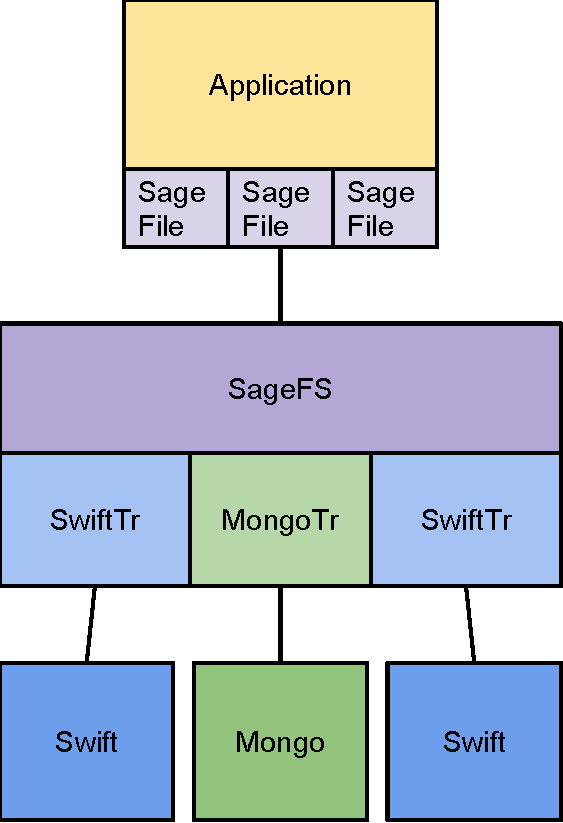
\includegraphics[scale=0.7]{figures/implementation}
\caption[Example Sage Deployment]{An Example of a possible Sage deployment with the current Implementation}
\label{fig:implementation}
\end{figure}


\section{File Objects}

We start looking at the filesystem by examining the actual file objects. There are two types of Sage file objects, SageMemFiles and SageDiskFiles.  Both classes inherit from the SageFile class, but SageMemFile also inherits from the StringIO class while the SageDiskFile inherits from the base Python file class. Figure \ref{fig:sagefile} shows the inheritance hierarchy of SageFiles. Subclassing StringIO allows SageMemFiles to reside as buffers in memory, excellent for smaller files that do not need to be put to disk. SageDiskFiles are written as temporary files on the client system. Temporary files are written to \textit{/tmp} by default, however the location is configurable.

\begin{figure}[h]
\centering
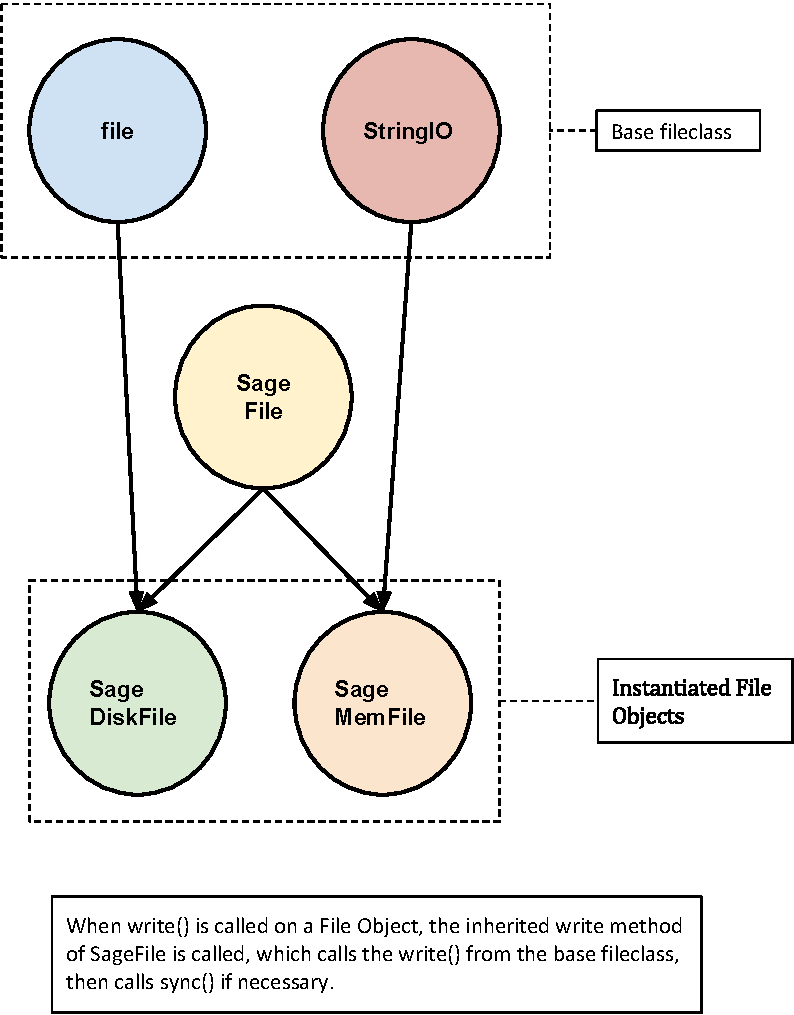
\includegraphics[scale=0.7]{figures/sagefile}
\caption{SageFile inheritance graph}
\label{fig:sagefile}
\end{figure}

The base SageFile object has a few key variables and methods that facilitate interaction with Sage. Each SageFile knows which backend it belongs to.  This information is used in the sync() method, which re-uploads (pushes) file contents into its backend. sync() can be called within an application, but it is also called within the write() family of methods for SageFile objects. If we take write() as an example, we see it takes three arguments as shown in Figure \ref{fig:sagefilewrite}.  The first argument \textit{self} is a reference to the calling object. Python makes this explicit, while in  a language like Java the self-reference `this' is always the first argument to a method,  but not explicitly stated in the method signature. The second argument \textit{arg} is the argument to the underlying file object's write() method. This argument contains the actual data to write to the file. The third is an optional flag indicating whether or not the file should call sync() at the end of the write operation. The flag is included in case we only want to update the local copy and not write back into the backend repository after every write (ie. cached writes). 

\begin{figure}[h]
\centering
\begin{lstlisting}

def write(self, arg, sync=True):
  """ Calls the underlying write function for the file.
  Will sync with remote storage by default, 
  will not if sync is False """
  self.fileclass.write(self, arg)
  if sync: self.sync()

\end{lstlisting}
\caption{SageFile write function}
\label{fig:sagefilewrite}
\end{figure}

Closing SageFiles also calls the sync() method. The close() method looks similar to write() except it only takes the optional \textit{sync} flag argument. When a file is closed, it is first synced back to its backend  repository, then removed from a local file cache within Sage. The file is only removed from the cache if sync() was successful so If an error occurs, the file will still reside in Sage and no data is lost. Of course if the \textit{sync} flas is \textit{false} then the file is simply removed from the cache. A special method for SageFiles called todisk() takes the file from Sage and persists it to the local system. This convenience method allows files to be easily taken from Sage.



\section{Backends}
\label{sec:backends}

Before we examine translator objects lets first take a look at the backend stores that translators connect to, and how Sage views them as filesystems. 

\subsection{Swift}

Swift is an object store system developed by OpenStack as an open source alternative to Amazon's S3. Clients interact with Swift's RESTful API through HTTP using PUT and GET to access files. Swift has two main types of nodes, storage that store data, and proxies that handle requests to Swift. The set of Swift processes on a given machine makes it a storage or proxy node, and in fact a single machine can be both a storage and proxy if all Swift processes are running on it. Swift distributes and replicates files across all storage nodes using structures called rings. Rings are abstractions over a set of values that Swift that maps to a set of storage nodes. Figure \ref{fig:swift} shows an object being placed within a Swift cluster. The object is sent through a partition function and placed onto Swift's object ring. The ring is broken into a number of partitions, each of which point to a set of storage nodes. The Proxy node handles the partitioning of the file based on the ring configuration and sends data to the storage nodes. The number of nodes a file is distributed to is called the replication factor of the cluster. All requests go through proxy nodes, so clients never directly contact storage nodes. A cluster can have multiple proxies, and each request goes to exactly one of them.

\begin{figure}[h]
\centering
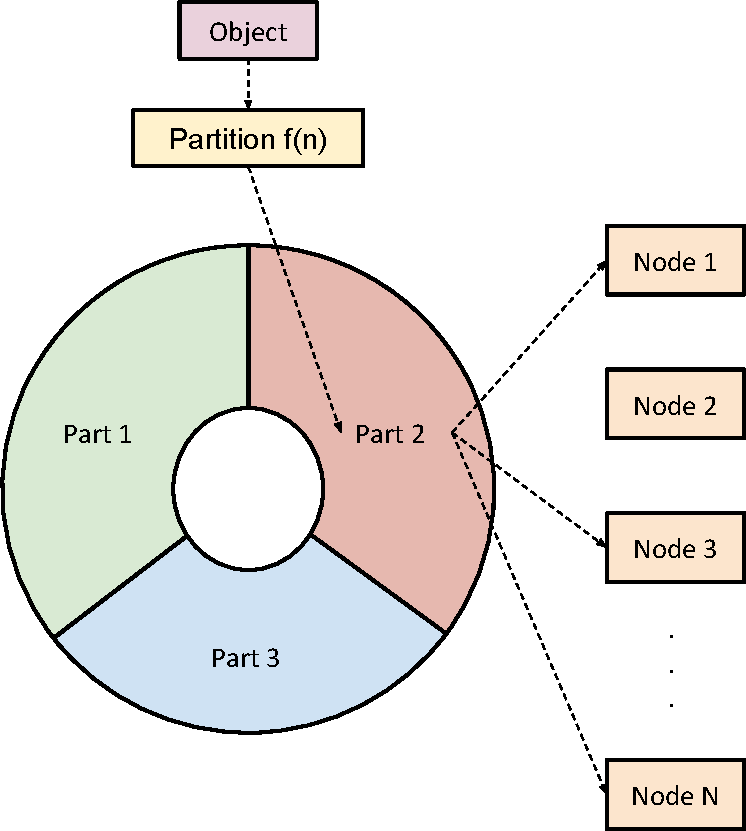
\includegraphics[scale=0.7]{figures/swiftrings}
\caption{The OpenStack Swift Ring Structure}
\label{fig:swift}
\end{figure}

Swift also contains accounts and containers which logically separate files into groups. In the Swift translator, I use accounts and containers to implement users and groups in Sage. Each account is a group, and each container is a different user. As a side note, the group implementation is incomplete in Sage as applications must interact with translators to view other users files. I use full paths to store files in Swift, but do not store directories. Directories are implied by file paths in the translator so if all files are removed in a given directory, the directory is removed as well. The Swift client allows partial name matching which I use to search for all files logically grouped in a directory. I do this by querying the path name (not including file name) as a substring. I use the swiftclient Python module to communicate with Swift specifically using the put\_object() and get\_object() function calls to upload and download data.


\subsection{MongoDB}

MongoDB is a database that uses document oriented storage to store objects. Documents are data structures that store information in key-value pairs. Documents are organized into collections to allow efficient querying and indexing. Data is stored as Binary JavaScript Object Notation (BSON), a superset of JavaScript Object Notation (JSON), which allows MongoDB to store arbitrary bytes of data. MongoDB can exist as a standalone database on one machine, or can be distributed in a cluster. When distributed, MongoDB has Config Servers that hold metadata, and Shards that house the data. A given document collection can be distributed across Shards much like disk striping. Config Server metadata is held in a config database that maps documents to Shards. Shards must contact Config Servers to access document metadata.

In the MongoDB translator, I make use of databases and collections to implement users and groups. Files are stored as key value pair documents, with the key being the full file path, and the value being the files binary data. In the document, I store path and file name as two separate fields as I want to be able to search for paths and partial paths when listing files. I use the Python module pymongo to communicate with MongoDB using the collection.insert() and collection.find\_one() functions to upload and download data.


\subsection{Local}

A very rough implementation exists to incorporate the local filesystem into Sage. Developed mostly for testing purposes, this translator is missing functionality other than reading and writing files. Files are created in the temporary directory \textit{/tmp/sage}, which acts as the root for the translator.

\section{Translator Objects}

Translator objects are Sage components that convert SageFS API calls into a set of backend calls to perform the actions of the API call in the backend. Translators must implement the methods upload(), open(), stat(), copy(), move(), list(), and remove(). Additionally the translator must keep a cache of open files. Files are downloaded from translators using the open() call. As we can see from the method signature in Figure \ref{fig:swifttropen} the open() call has one required parameter and two optional; \textit{create} which defaults to \textit{false}, and \textit{inmem} which defaults to \textit{true}. If the file specified at \textit{path} does not exist in Swift, and \textit{create} is \textit{true}, then an empty file will be created in the translators cache. The file is not  created in the backend until its sync() method is called. The second argument specifies whether the file should reside in memory or on disk on the local system. If \textit{inmem} is \textit{true} then the file is opened as a SageMemFile, otherwise it is opened as a SageDiskFile. If open() is called on an already open file, the translator returns the open file descriptor for the file, not a new one. This is done to avoid having two sets of the same file downloaded, and the consistency issues associated with that. It would be possible to implement file pointers within the SageFile object which would allow two file descriptors for the same file. However, this functionality does not exist in the current implementation.

\begin{figure}[h]
\begin{lstlisting}

def open(self, path, create=False, inmem=True):

\end{lstlisting}
\caption{The Swift Translators open() Method Signature}
\label{fig:swifttropen}
\end{figure}

The rest of the translator is convenience methods or methods for connecting to the backend repository. For example, SwiftTr holds all the relevant info to connect to Swift, as well as interface back with SageFS. The actual Swift repository knows nothing about the translator and communicates via the RESTful interface provided. Using REST commands makes implementing translators simple since the six methods just have to be translated into appropriate REST calls. The translator also converts filesystem paths into actual locations in the backend store. Since both Swift and MongoDB are not natural filesystems, paths and directories are faked within them. To do this I simply incorporate the full path as the actual name of the file in the backend store. These paths allow Sage to separate files into a virtual directory tree, and query based on a fragment of the path. Both Swift and MongoDB translators can handle queries on partial paths.


\section{SageFS}

The SageFS object is the central component of Sage and implements the seven API methods (open(), remove(), list(), stat(), copy(), move(), and upload()) exported for use by applications. Of course, an application could use any part of the sagefs.py Python module, but the intended use is to interact with the SageFS object. The SageFS object holds a dictionary mapping names to translator objects, as well as a list of all the available backend repositories called sites. The SageFS constructor and connect\_to\_filesystem() methods are shown in Figure \ref{fig:sagefscode}. We see the \textit{filesystems} dictionary is initially  empty. The actual translator objects are not instantiated until the site is accessed within Sage. When a site is accessed for the first time, Sages connect\_to\_filesystem() method is called which creates a translator object and stores the object in the \textit{filesystems} dictionary. The lists \textit{swiftrepos} and \textit{mongorepos} hold the backend host info required to connect to the backend, which is examined later in Section \ref{sec:config}.

Currently, we see only two translators in connect\_to\_filesystem(), identified as SwiftFS and MongoFS in the code for legacy reasons. If I wanted to implement more translators for Sage, the connect\_to\_filesystem() method would need to be modified to handle the creation of these new translator objects. I could create a new list of backend hosts for the new repository type in the SageFS object, however this approach is not very scalable. A more scalable approach would be to make the SageFS constructor take a dictionary mapping site names to the constructor method of the appropriate backend instead of lists of site names for each backend individually. This way connect\_to\_filesystem() can index into the site name-constructor map and call the correct translators constructor without going through a long chain of if/else statements.

\begin{figure}[h]
\begin{lstlisting}

class SageFS():
  """ The main filesystem object which holds a collection of SwiftFS
  and MongoFS objects. Connections are only established when they
  are used the first time. The SageFS object is designed to be the 
  only object that must be explicitly created to use the SageFS. """

  def __init__(self, swiftrepos=hosts.swift, mongorepos=hosts.mongo):
    self.filesystems = {}
    self.swiftrepos = swiftrepos
    self.mongorepos = mongorepos
    self.sites = self.swiftrepos.keys() + self.mongorepos.keys()

  def connect_to_filesystem(self, site):
    """ Creates a translator object if we correctly connected """
    fs = None
    if site in self.swiftrepos.keys():
      repo = self.swiftrepos[site]
      fs = SwiftFS(repo.get_authv1_url(), repo.group, repo.user, repo.key)
    elif site in self.mongorepos.keys():
      repo = self.mongorepos[site]
      fs = MongoFS(repo.host, repo.port, repo.database, repo.collection)
    else: raise SageFSException('No host matches site %s' % (site))
    self.filesystems[site] = fs
    return fs

\end{lstlisting}
\caption[SageFS Constructor]{The SageFS constructor and connect\_to\_filesystem methods. The class instance variable self.filesystems holds the SageFS objects collection of translators.}
\label{fig:sagefscode}
\end{figure}


Now let us examine the API calls in the SageFS object. From a high level, when a method is called on a SageFS object, the method first chooses the correct translator based on the file placement logic, then calls the underlying translators method to perform the call. In the current implementation file placement is done by path name via the method split\_location\_from\_path() (which is easily extended as discussed in Chapter \ref{chapter:arch} and Chapter \ref{chapter:conc}). The method returns an index into SageFSs \textit{filesystem} dictionary, which is then used to grab the appropriate translator to perform the method call. Some methods operate over multiple translators. stat() and list() can be used to probe all backends, while copy() and move() may involve two different backends. To get a better understanding of how methods are handed to translators in SageFS, let us examine the copy() method, shown in Figure \ref{fig:sagecopy}. While copy() it is the most complicated call in Sage, it demonstrates the power of the aggregation of multiple translators in SageFS. 

\begin{figure}[h]
\begin{lstlisting}

def copy(self, origpath, newpath, overwrite=False):
  """ Copy a file from 'origpath' to 'newpath'.
  Will not overwrite unless specified """
  if origpath == newpath: return
  origlocation, origresource = self.split_location_from_path(origpath)
  newlocation, newresource = self.split_location_from_path(newpath)
  origfs = self.get_filesystem(origlocation)
  if origlocation == newlocation:
    # if both resources use the same fs use the fs's copy
    origfs.copy(origresource, newresource, overwrite)
    return
  newfs = self.get_filesystem(newlocation)
  # check to see if we are overwriting anything
  if not overwrite and newfs.file_exists(newresource):
    raise SageFSFileExistsException('File %s already exists' % (newpath))
  local = True
  if origresource not in origfs.localfiles:
    # make sure the orig file is local to its fs
    local = False
    origfs.open(origresource)
  origfd = origfs.localfiles[origresource]
  # upload as a new resource
  try: newfs.upload(newresource, origfd)
  except swiftclient.client.ClientException as e:
    raise SageFSException('HTTP Error: %s - %s' 
               % (e.http_status, e.http_reason))
  if not local: origfd.close() 

\end{lstlisting}
\caption{The SageFS API copy method}
\label{fig:sagecopy}
\end{figure}

The method takes three arguments; \textit{origpath} the path to the original file to copy, \textit{newpath} the desired path for the new copy, and an optional argument \textit{overwrite} that specifies whether the copy should overwrite an existing file if it exists. copy() first checks if we are trying to copy to the same path to avoid redundant work, if we actually need to copy then we determine which translators the old file and new file belong to (or should belong to). If the copies will use the same translator we forward the copy() call to the containing translator. If they do not use the same translator we continue. We check if a file exists at the new location and \textit{overwrite} is \textit{false}. If so raise an exception saying that the file already exists. If no exception is raised we check to see if the SageFile is open in Sage. If not then we open the file and set the variable \textit{local} to \textit{false}. The value of \textit{local} tells us whether we should close the file after the copy is complete as we want to keep the set of opened files the same as when the copy was started. We then call upload on the new translator, giving the new file name and the old files data as arguments. This makes a copy of the file in the new backend without opening the file that ensures the set of open files in the new translator remains unchanged. We finally close the original file if it was not local to the original translator as again we want the set of open files to remain unchanged.

SageFS uses its own exceptions for error handling. As we can see in Figure \ref{fig:sagecopy} the Swift exception \textit{swiftclient.client.ClientException} is converted into a \textit{SageFSException}. All errors coming from client libraries are converted into \textit{SageFSExceptions} as well as filesystem errors such as trying to overwrite a file or open a non existent file.


\section{Configuration}
\label{sec:config}

SageFS takes a collection of repositories as arguments, which can either be passed to the constructor or defined in the configuration file hosts.py included in SageFS. Sage configuration is done with a dictionary of Host objects, in this case SwiftHosts and MongoHosts. These objects define connection parameters to each of the backends and a key which identifies the backend. As an example Figure \ref{fig:swiftconfig} shows a configuration dictionary for Swift backends. The dictionary shown is passed by default to the SageFS constructor previously shown in Figure \ref{fig:sagefscode}. The dictionary contains three keys \textit{vic}, \textit{tor}, and \textit{carl} that map to three SwiftHost objects. A SiwftHost object defines parameters to connect to a Swift repository. Here we see the IP addresses of three Swift clusters used as Sage backends. The dictionary shown was used in the deployment of SageFS for the genome searching case study described in Chapter \ref{chapter:exp}. SageFS uses the hosts in the configuraton file by default, but can also be passed dictionaries in the constructor.

\begin{figure}[h]
\begin{lstlisting}

swift = {
  'vic':SwiftHost('142.104.17.135', 'admin', 'system', 'sagefs'),
  'tor':SwiftHost('142.150.208.220', 'admin', 'system', 'sagefs'),
  'carl':SwiftHost('134.117.57.138', 'admin', 'system', 'sagefs')
}

\end{lstlisting}
\caption{Configuration dictionary for Swift backends}
\label{fig:swiftconfig}
\end{figure}

Currently, the SwiftHost and MongoHost objects are the only SageHost objects defined in hosts.py. SwiftHosts require a hostname (or IP address), user, group, and key to connect to a Swift backend, while MongoHosts require a hostname, database name, and collection name. Translators use these parameters to authenticate with their respective backend.

\section{Using Sage}

To use Sage from a client perspective we only need to import the sagefs Python module into a Python project. This allows us to use SageFS with the default backends as the default user provided in the hosts.py configuration file. As discussed previously, to use different backends we can either modify hosts.py or pass in our own dictionary. One thing to note is that if we define a filesystem that does not exist or does not accept the connection parameters we provided, SageFS will not fail until it tries to access the dysfunctional backend. We can also define a backend twice with a different dictionary key. SageFS will think the two backends are different, create two translators, and allow file operations on both. If we open the same file in both backends, Sage will have two copies of the same file. If we write different things to each copy, the copy with the last sync() operation will remain in the backend.

\begin{figure}[h]
\begin{lstlisting}

import sagefs
fs = sagefs.SageFS()
__builtins__.open = fs.open

\end{lstlisting}
\caption[Builtin Open Overwrite]{An interesting hack to overwrite Pythons builtin open call to use Sage's instead.}
\label{fig:sagepythonhack}
\end{figure}

Once the module has been imported we create a SageFS object which allows us to perform operations on the filesystem. To interact with files we call the SageFS objects open() which returns a SageFile object, which is then used normally like any other Python file object. In fact, if we wanted to use Sage in an existing Python application we could accomplish it in a few lines of code as shown in Figure \ref{fig:sagepythonhack}. We would only need to import the sagefs module, instantiate a SageFS object, then overwrite Python's builtin open() function with Sages open(). After doing this all calls to open() will go through Sage and all file objects will be SageFiles. We could also go a step further and define a closure around Sages open() to extract information about the file. The information could be passed through open() to allow interesting file placements with a custom file placement function. Of course, other operations from other Python modules that utilize the builtin open(), or modules that manipulate the local filesystem will remain unchanged so more work may be required on a more complicated system. Additionally Sages open() will throw different exceptions than the builtin so applications could suffer from unexpected exceptions.

The client side of SageFS is implemented as a Python package, which can be downloaded from github. I also developed server side deployment scripts for Swift, which will install and configure Swift on a cluster of machines (either Ubuntu or Fedora) using the Fabric Python module. Once the Swift cluster (or clusters) are running, the hosts.py file can be edited to make the clusters the default backends, or backends can be passes as a dictionary to a SageFS object.